%!TEX root = ../paper.tex


\section{Impact of Device Performance} \label{intro}

%\mallesh{Large fraction of people in developing regions use cheap phones, though large fraction of networks there may provide adequate speed \cite{mobilephones,contreras2017patents,jioplans1,jioplans2}}

While mobile smartphones have now penetrated 
a significant fraction of world population, the devices 
vary widely in terms of cost and performance. 
%The mobile device penetration is characterized by a large diversity in smartphone/mobile devices to suit the needs for diverse users.
For example, the smartphones in the market 
range from $\approx$\$50 to $\approx$\$1000~\cite{mobilephones, contreras2017patents}, and the cost 
largely depends on the hardware specifications. 
For example, a \$600 phone such as OnePlus5 has 8 cores, running upto 2.4\,Ghz clock and 6\,GB RAM, while a cheaper \$60 phone (e.g., Dell Venue Pro) only has 2 cores with up to 1\,GHz clock and 512\,MB RAM. 

However, the impact of the hardware specs
on the performance of mobile Internet applications is not well-studied. A large fraction of past research on mobile Internet performance has focused on the effect of the {\em network} on the applications~\cite{butkiewicz2015klotski, kelton2017improving, singh2015flexiweb, Ruamviboonsuk:2017:VAM:3098822.3098851, Shafiqund, Xiaodash2m, chen2016effective} but not 
the device. Some studies do address the compute performance of mobile Internet applications~\cite{zhu2017optimizing,jones2009parallelizing,mai2012case}, but the underlying
technologies developed are more suited for higher end devices. 

%\todo{Can we say these are for high-end devices? or that they only look at energy-- There has been work on improving the compute performance of mobile Internet applications~\cite{kilgard2012gpu,zhu2017optimizing,jones2009parallelizing, mai2012case}, but these works do not address the network performance directly.} \mallesh{Yes, 28 and 32 are browser parallelization work. 30 is gpu related work. 51 is energy specific work.}

Given that a large fraction of mobile
users in developing regions (62\%-68\% by some 
account \cite{unity}) uses smartphones with relatively
less expensive lower end hardware, it is important
to understand the impact of the device hardware on the 
performance of the mobile apps. In fact, with the increased 4G penetration, network speed is no longer the bottleneck in many developing countries~\cite{mobilephones,contreras2017patents,jioplans1,jioplans2}.  Our measurements show that mobile Web page loads on two popular phones in India, Intex Amaze 4 ($\approx$\$60) and Gionee ($\approx$\$150) are $5\times$ to $3\times$ worse, respectively, compared to Web page loads on Google Pixel2 ($\approx$\$700) under the same network conditions (\S\ref{sec:motivation}). 
This underscores the importance of studying the influence of the device hardware
on the performance and explore ways to improve the mobile web experience on lower end hardware. 
%This is largely because unlike laptops, mobile Internet applications are often compute-bound and not network-bound~\cite{nejati2016depth}.  

In this paper, we focus on three types of mobile Internet applications:  {\em (i)} Web browsing, {\em (ii)} video streaming, and {\em (iii)} video telephony. We study performance in terms of Quality of Experience (QoE) and energy. We especially focus on how the {\em CPU clock frequency} impacts performance 
given that the clock frequency
has the most impact on the performance
among other aspects of the specification (\S\ref{sec:impact_cpu}).% varies  important resource that changes across low-end and high-end devices as the representative   
%However, our experiments show that the CPU clock has the most impact on application performance among these resources (\S\ref{sec:impact_cpu}). 
%For example, \todo{write something here to convince that this is the case}.
%\mallesh{We show this by measuring Web performance under different clock, memory and GPU conditions on Nexus4 phone. We find a low memory of 512MB RAM has an impact of 4 seconds increase in PLT while a lower clock of 384Mhz shows 11 seconds increase in PLT. We also measure the impact of disabling GPU, which has a 0.5 seconds difference from normal PLT which is 3.5 seconds. This shows that Clock frequency has an exponential increase in PLT.}
%The second problem that we solve is curating different hardware conditions. It is difficult to measure the application performance on various smartphones available in the market. So we take the approach of emulating these diverse smartphones by using a representative hardware parameter of smartphones. In our research, we find clock frequency of CPU is a key factor in application performance. Clock frequency directly determines the amount time required for certain computation. Hence, we use clock frequency parameter to emulate different smartphones because we find smartphones with clock frequency ranging from 300Mhz to 2.4Ghz in the market. We change the clock frequency with the help of clock frequency scaling algorithm called governor (Userspace) provided by Andriod. This allows us to fix the CPU clock on a smartphone.
%The QoE of an Internet application depends on several factors apart from the device hardware, including the network condition, the server, and other factors in the data delivery path. The problem is these factors are interdependent on one another (for example, impact of hardware on network apart from application computation). 

One of our key findings is that a slow CPU speeds not only affects compute performance, but has a second-order effect on the network
performance. In our measurements, for example, the TCP performance drops more than 20\,Mbps, 
when the CPU clock of the phone drops from 1512\,Mhz to 384\,Mhz. This is owing to 
the fact that a slower clock
increases TCP processing delays by as much 
as $\approx$12\,ms.
%In our experiments, the time between when the packet reached the kernel to when it reached the application differs by as much as 11ms between a slow and a fast CPU. 
The implication is that the application is doubly 
impacted by the slower clock that slows
down both the network latency/throughput as well as the compute 
performance inside the application. 
%since Internet application performance depends on both the network and the compute performance. 
% to low clock frequencies---affecting both compute and network. Application performance is a combination of the network performance, involving loading network objects, and computation performance, involving processing. 

Our goal now is in {\em isolating} the effect of CPU clock on the network and the compute activities of the application. This isolation is critical to shed light on how the application 
performance can be improved for low-end devices: should the optimization focus on improving the TCP packet processing or the application compute? While straightforward for video applications, for Web browsing, this isolation is challenging.  
Loading of Web objects, a network process, and processing of these objects, a compute process, are intertwined during the page load process and cannot be cleanly separated. To this end, we leverage the WProf tool~\cite{wang2013demystifying,nejati2016depth} that breaks down the Web page load process into network and compute processes on the critical path. The key findings of our study are: %In the case of video applications, we isolate the effect of network and compute by

% using  is challenging because Isolate the network and compute for video applications bIsolating the effect of network is more straightforward for video applications, since there are no dependencies. However, isolating the effect of compute is harder because many video applications are not open. Instead, we experiment with the open source VLC player to study the compute performance in detail. \todo{this para does not have any message.}


%because loading the Web objects (a network process) and processing the Web objects (a compute process) cannot be decoupled easily due to dependencies~\cite{wang2013demystifying,nejati2016depth}. To this end, we leverage the WProf tool that uses dependency analysis to divide the application performance into network and compute components on the critical path. Using the dependency and critical path analysis, we `fix' either the network or the compute component of the page load 
%to be constant and study the effect of CPU clock on the other component. 




% \todo{what do we do?} \mallesh{ For video applications, it difficult to isolate the effect of clock on network and compute on our applications( i.e, YouTube and Skype) because of lack of open source. In another way, for video applications it is more straightforward because there is no such dependencies as in Web. So, we use an open source VLC player to decouple the impact of clock on network and compute. To isolate compute, we play a video locally without any network involvement and measure the video decoding performance. To isolate network, we tap the source code and measure the number of video packets received before video decoding a particular packet.}

%Therefore, we need to isolate the effect of hardware on application performance from network to find the individual impact. But the challenge in isolating the effect of hardware is: First, the applications are different and require separate mechanism in isolating hardware from network. Second, for applications such as Web browsing, we decouple the network from compute by scheduling (replaying) object downloads by keeping the compute constant. But, this requires us to preserve the dependencies and computaion of live pages. We use WProf to preserve the dependencies.
%\aruna{We need to say something concrete here. Simply saying, we keep one parameter constant is not enough. Think of what is the most interesting challenge in isolating the effect of hardware}


%\aruna{again, extremely vague. What does "such as" mean, what exactly are you changing, why did you choose this parameters. How exactly are you doing this study. We need a lot more details here . For instance, why is clock frequency what is being changed? }.


\begin{itemize}    

   \item {\bf Mobile Web performance is significantly affected by slow clocks:} Web page loads slow down by a
    factor of 5 on average when CPU clock speed reduces from 1512 Mhz to 384 Mhz. This slow down is both because of compute processing delays and the second-order effect in network processing. Our isolation experiments show that compute processing is more of a bottleneck under slow CPU speeds, accounting for over 60\% of the 
    page load time. Within the compute activities, Javascript evaluation is affected most by 
    the CPU slow down, and rendering and painting are affected the least.
 
 %  the web page load slowed down by an average of 6 times across XXX Web pages, even when the network condition is held a constant. Under slow CPU clock, the processing of the Web objects slowed down, but the network loading is also affected because of the second-order effect described earlier. Using our isolation technique, we find that compute accounts for XXX of the slow down under low clocks. This result suggests that improving Web performance for low-end phones should focus on improving the performance of compute. 
   
   %The Web page load process consists of both network activities for loading objects, and compute activities for parsing HTML, running scripts, and rendering. Reducing CPU speeds both affects the compute activities directly, and the network downloads through the second order effect described earlier. To isolate this, we build an emulator which schedules object downloads by keeping the compute the constant. While scheduling object downloads, we preserve the dependencies captured using WProf tool. 

    \item {\bf A slow clock does not significantly affect video streaming because of offloading and pre-fetching:} 
    The QoE of video streaming is largely unaffected by slow CPU speeds, despite video streaming being a compute-intensive application. By isolating the impact of compute and network, we find that this paradox is because of two reasons. From the compute standpoint, 
     streaming applications use special hardware decoders, even available on low-end phones, to process video data rather than decode on the CPU.   %(e.g, \texttt{OMX.sprd.h264.decoder}). 
    From the networking standpoint, streaming applications pre-fetch enough data and are unaffected by the second-order network slow-downs caused by slow CPU. 
    %Video streaming applications have two key QoE metrics, the startup latency and the stall rate. The startup latency, which is the time when the video can start streaming, does increase under slow clocks. However, after this initial startup, video streaming applications are not adversely affected by slow clocks. Using isolation, we find that varying the clock frequency has no effect on compute. 
    
    %Clock frequencies {\em do} affect the network performance of video streaming, but this effect is masked by the read-ahead buffer since streaming applications prefetch frames. \newline%, and the stall rate is affected only if new data is not prefetched in time, which did not occur even under low clocks. 
    
  % Unlike streaming, video telephony cannot prefetch frames because of its interactive nature. Therefore the performance of telephony is impacted by slow clocks because of its second-order effect on the network. %The bitrate and framerate metrics reduces by 42\% and 33\% under low CPU clocks. 
   %However, similar to streaming, telephony applications offloads computation to a hardware accelerator; as a result, slowing down the clock has little effect on the compute component.
    
      %Andriod that significantly reduces the effect of CPU. But, we observe greater impact of clock on Skype eventhough it has hardware accelerated video decoding. This is due to the second-order effect of hardware on network. This effect is vanished in streaming because of read-ahead (prefetch) capability. We isolate this second-order effect using an open source Andriod VLC player. To isolate network, we locally play videos and measure QoE (i.e, Fps and stall ratio) which has only compute impact. To isolate compute, we ignore video decoding and measure the start-up latency and number of segments in the frame buffer, which has only network impact.

 \item {\bf  Increasing CPU speeds beyond a inflection point has poor performance/power trade-off:} For all three applications, increasing  CPU speeds significantly increases energy consumption. However, the corresponding improvement in performance beyond a point is not commensurate with the energy cost. 

 \item {\bf Leveraging hardware offloading is a promising approach to improving Web performance under slow CPU clock:}  Similar to the hardware offloading techniques used in video applications, offloading Javascript evaluation to a low-power DSP can potentially improve Web performance. Our preliminary 
 analysis with offloading only regular expression evaluations
shows that the improvement can be as much as 18\% in page load time along with a $4\times$ 
improvement in power consumption. %\todo{check the numbers.} 
 %\todo{this needs to be revisited to make sure it is still true.}
 
%\todo{Not sure if we should anything about energy}
  %  Therefore, as we observe mobile browsing has severe effect of clock, we present different strategies to improve web performance in terms of compute. First, we measure emulated page loads under DOM parallelization. We replay the object downloads by emulating the computation activities such as scripting and parsing in parallel. We also experiment with scale-up of compute power and emulate pageloads under such scenarios. This gives a maximum of 5 seconds reduction in PLT. Second, we offload certain computation of Javascript to DSP processor which is available on most of the smartphones and often underutilized. We find decent ($>$2seconds) improvements in pageloads under low CPU clock. We also observed energy consumption of DSP much lower (20\%) compared to CPU. Improving web performance from the second-order effect is out of scope. 

\end{itemize}

%We also study energy consumption since we find that the applications consume power very differently. For example, video streaming and telephony have linearly increasing energy consumption with clock. But, in case of Web browsing, the energy consumption is more at low clock (384Mhz, 2.5Joules) gradually decreasing till 594Mhz (2Joules) then starts increasing drastically with the increase in clock. This descripancy is becuase the eventhough low clock has low power consumption, it has high pageload time ($>$10 seconds), and thus the overall energy consumption is high.

%Summary: We find mobile browsing has a non-linear impact of clock while other applications has a linear impact. Video applications also has only second-order effect because of computation offloading to co-processors. Web browsing has both computation overhead and second-order effect of hardware on network. We try to solve computation effect by offloading certain Javascript computation to DSP.

\begin{figure*}
    \begin{subfigure}[b]{0.33\textwidth}
        \centering
        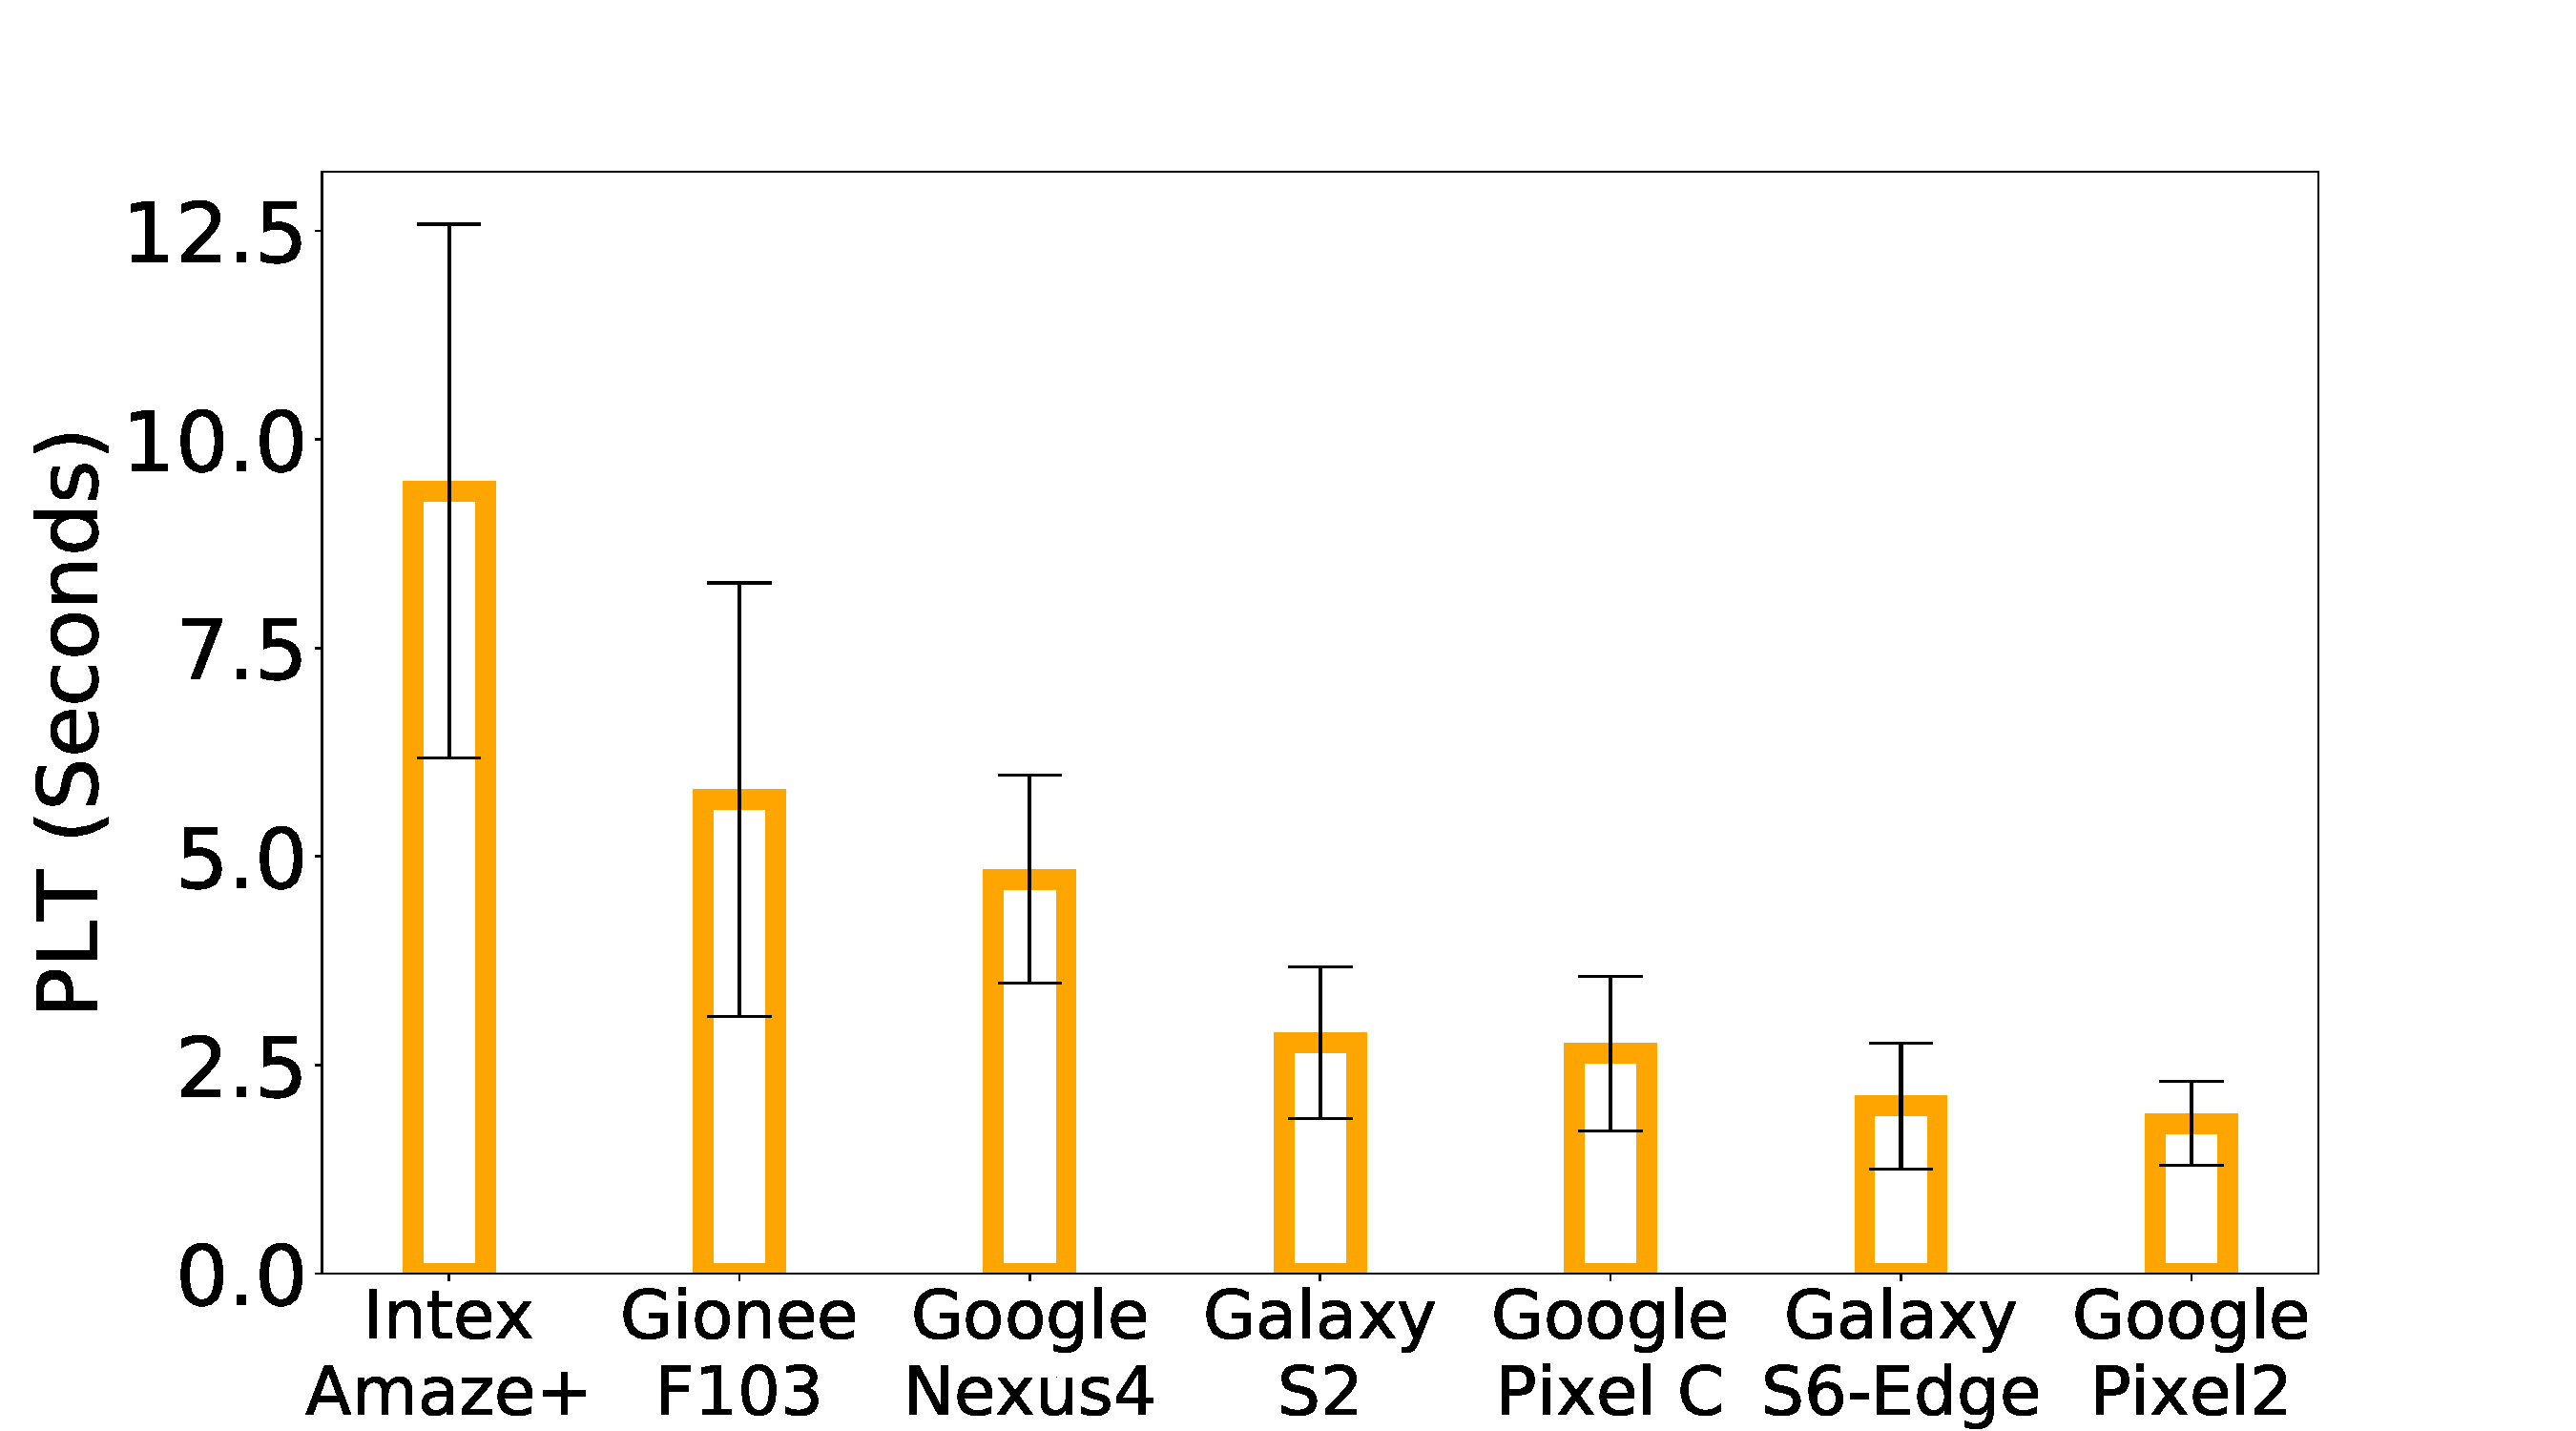
\includegraphics[width=1\linewidth]{sections/device-work/plt-devices}
        \caption{Content and Motion}
    \end{subfigure}
    \begin{subfigure}[b]{0.33\textwidth}
        \centering
        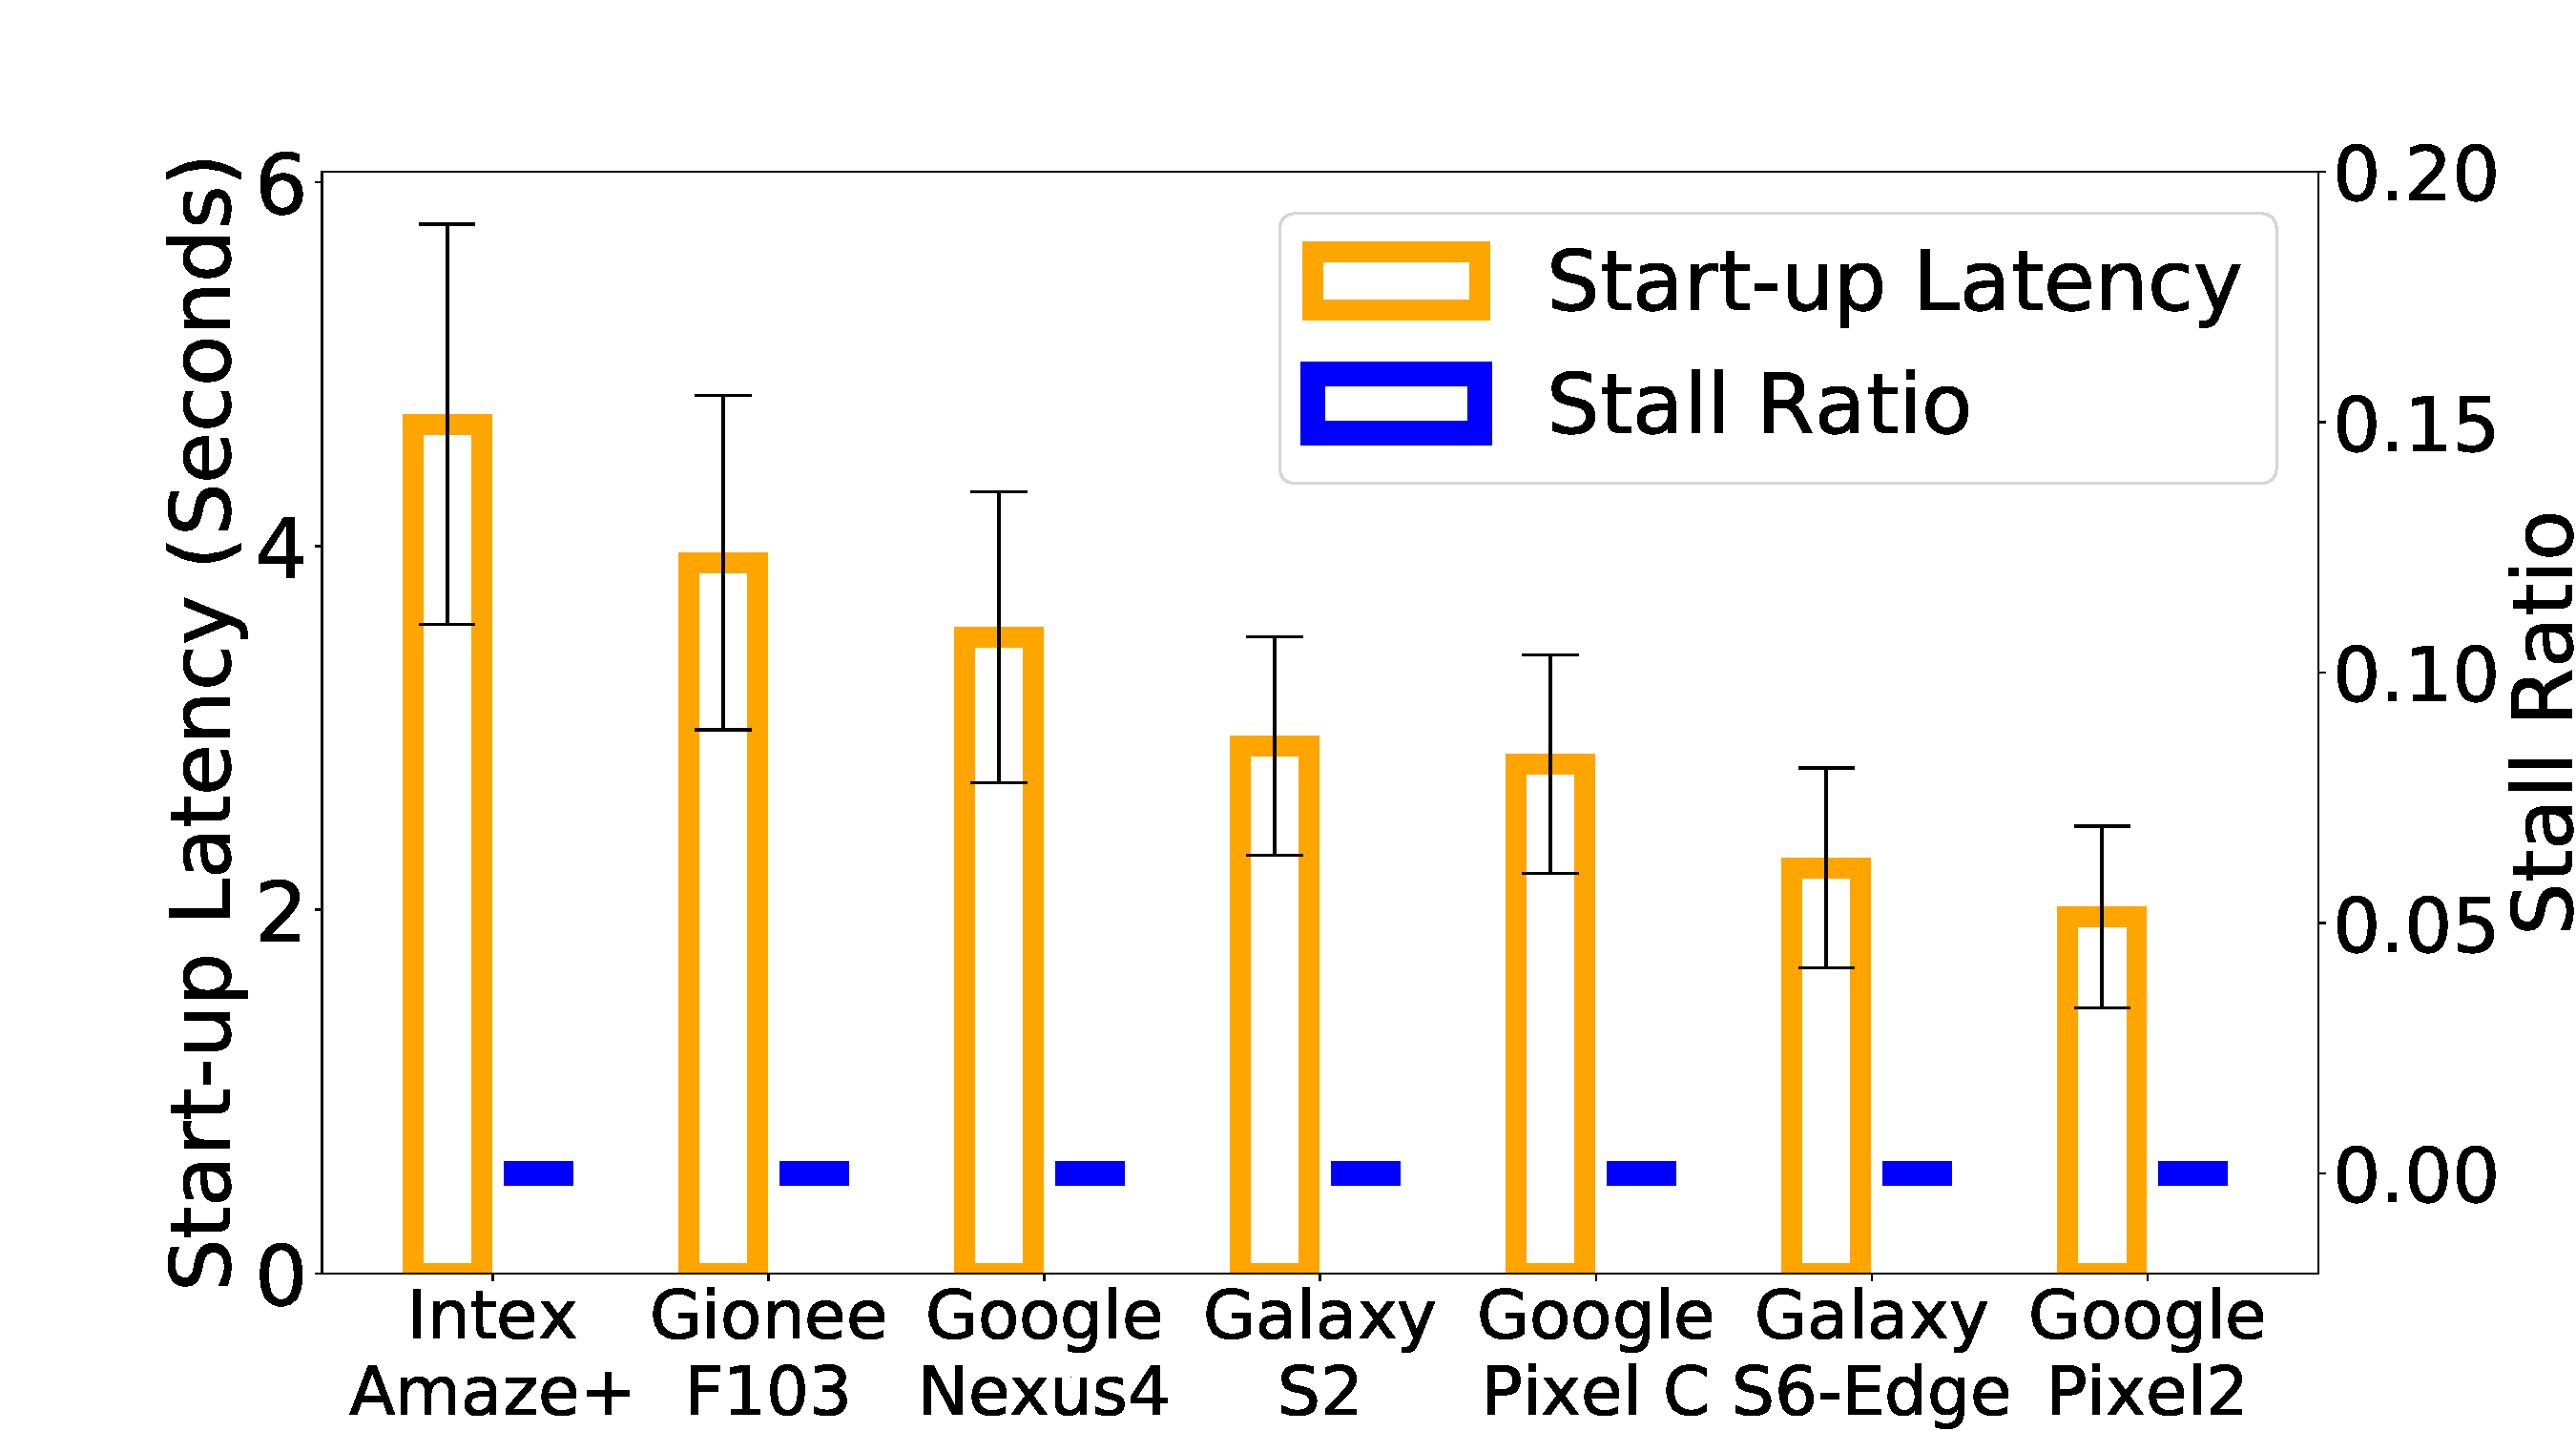
\includegraphics[width=1\linewidth]{sections/device-work/youtube-motivation}
        \caption{Applications}
    \end{subfigure}%
    \begin{subfigure}[b]{0.33\textwidth}
        \centering
        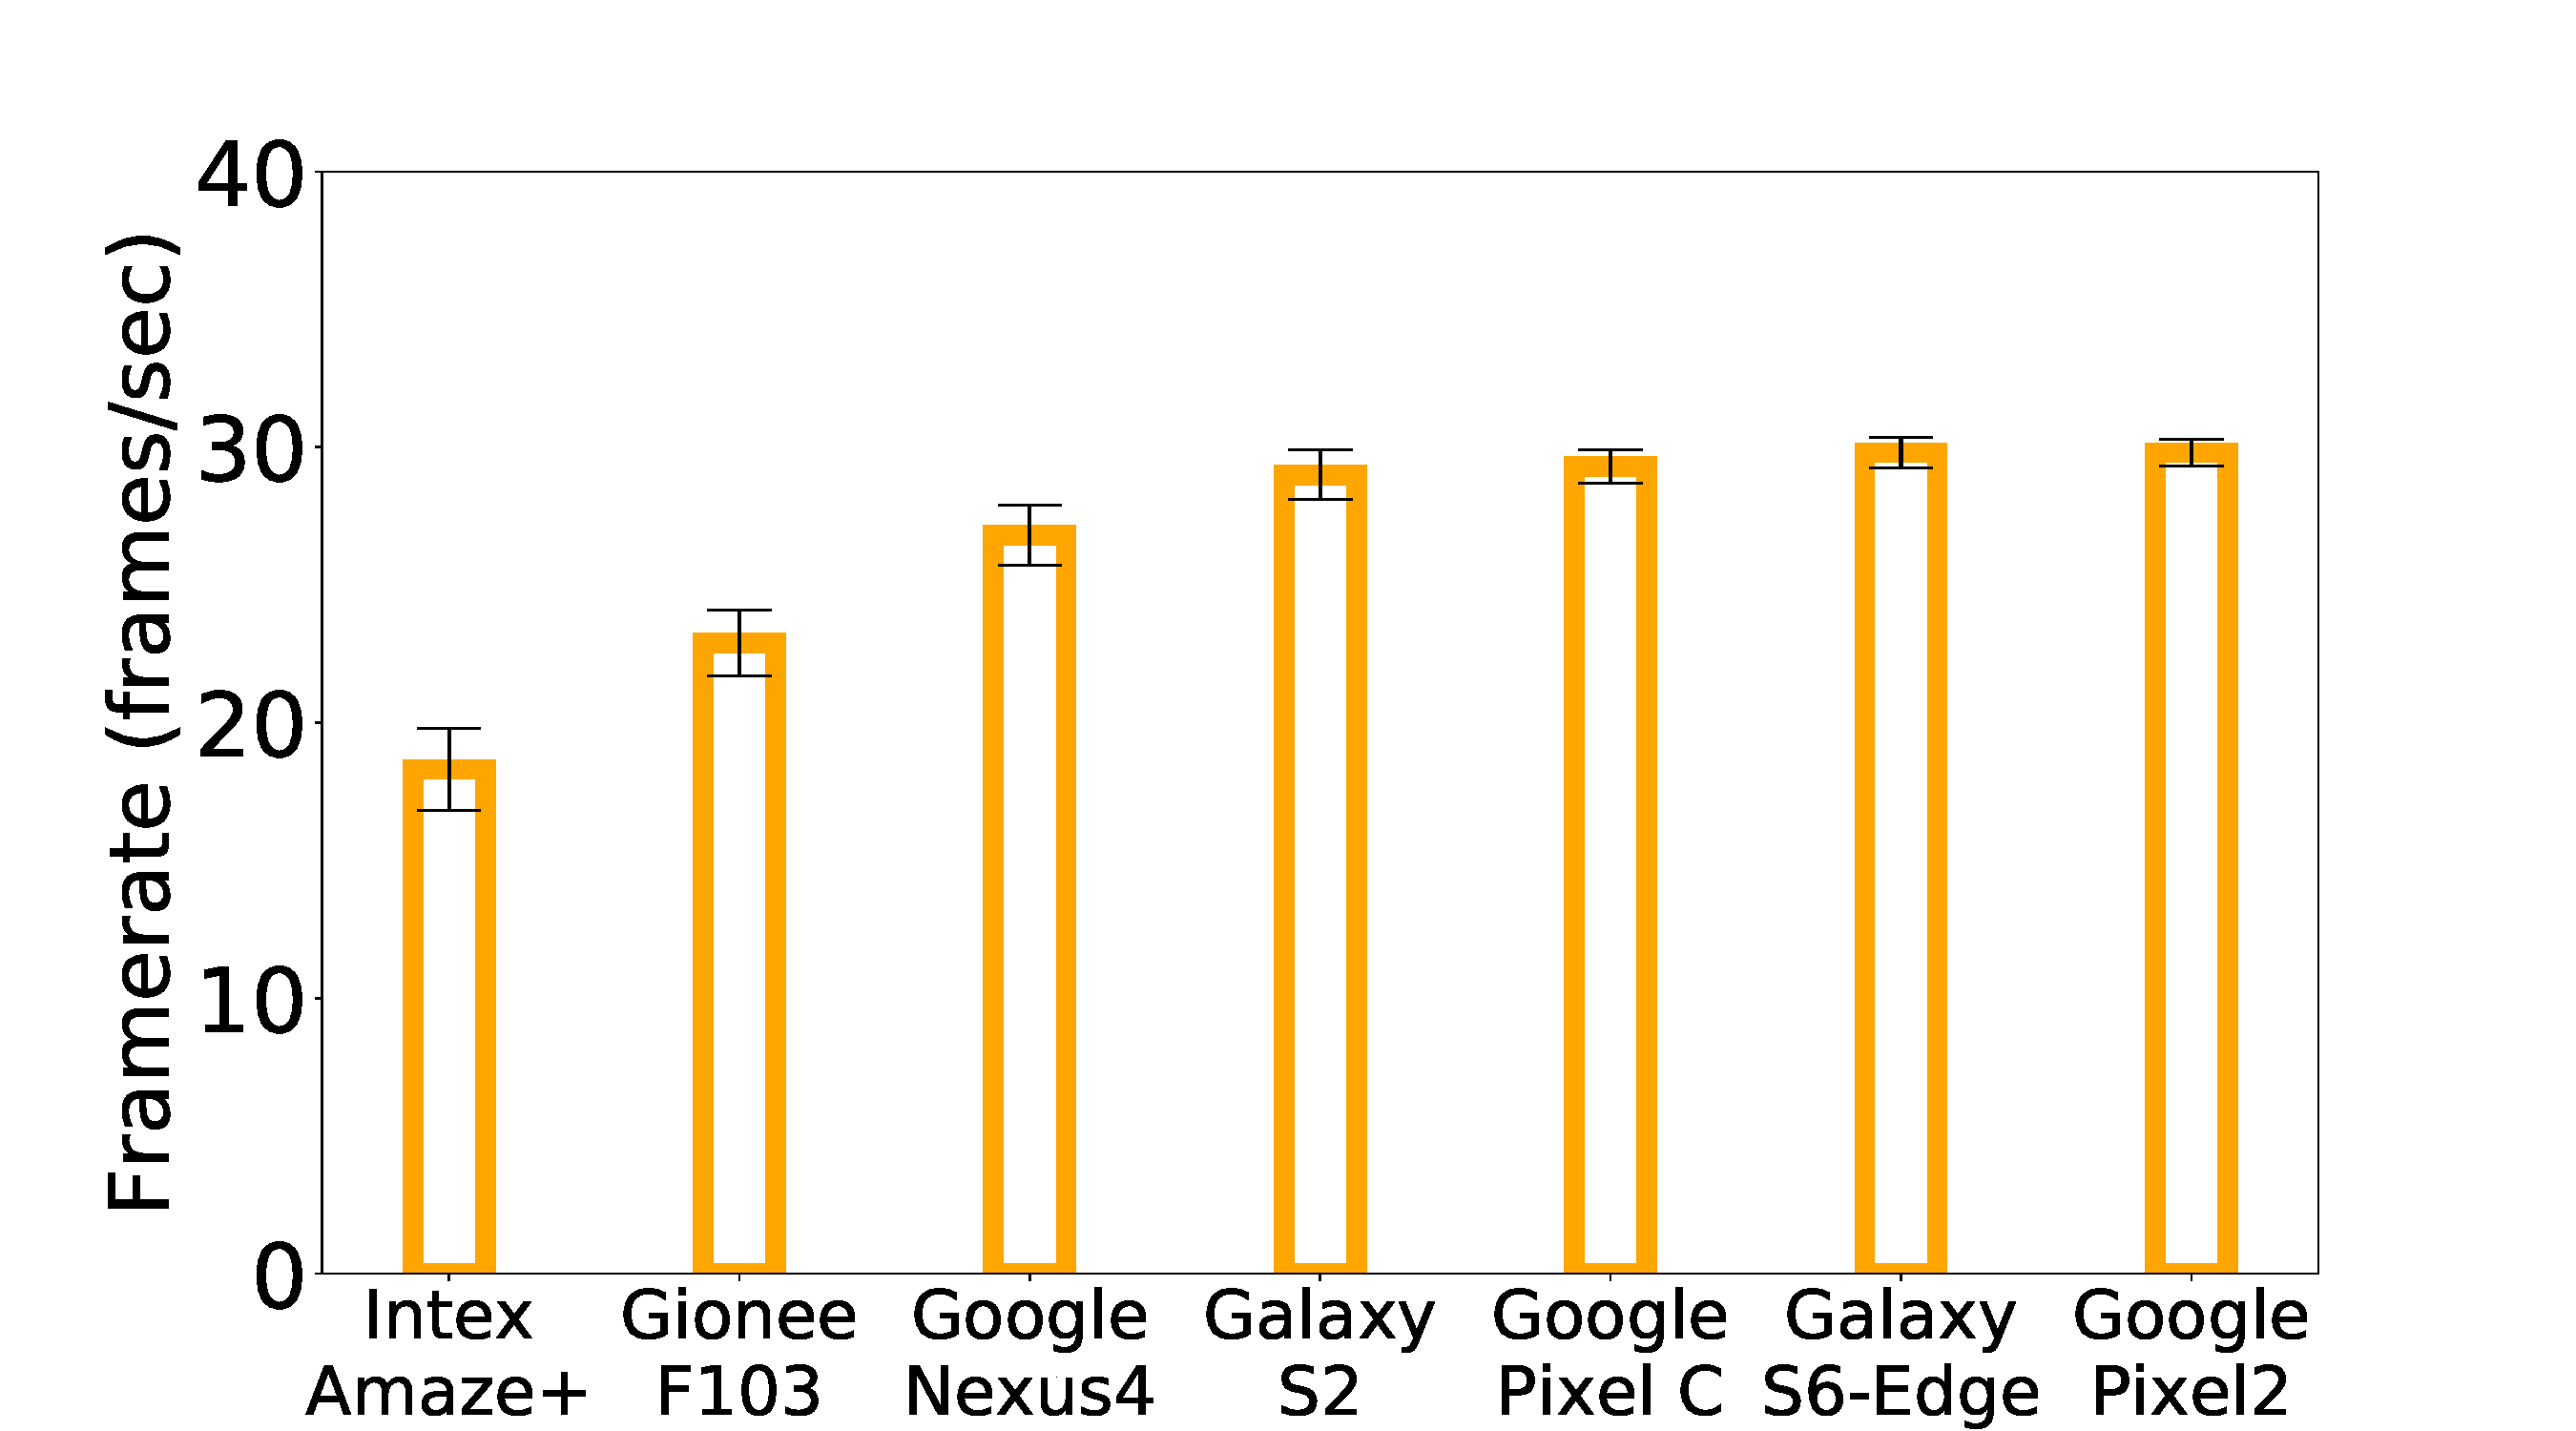
\includegraphics[width=1\linewidth]{sections/device-work/skype-motivation}
        \caption{Devices}
    \end{subfigure}
     \vspace*{-1em}
\end{figure*}



%\begin{figure*}[h!]
%     \subfloat[Web Browsing]{%
%       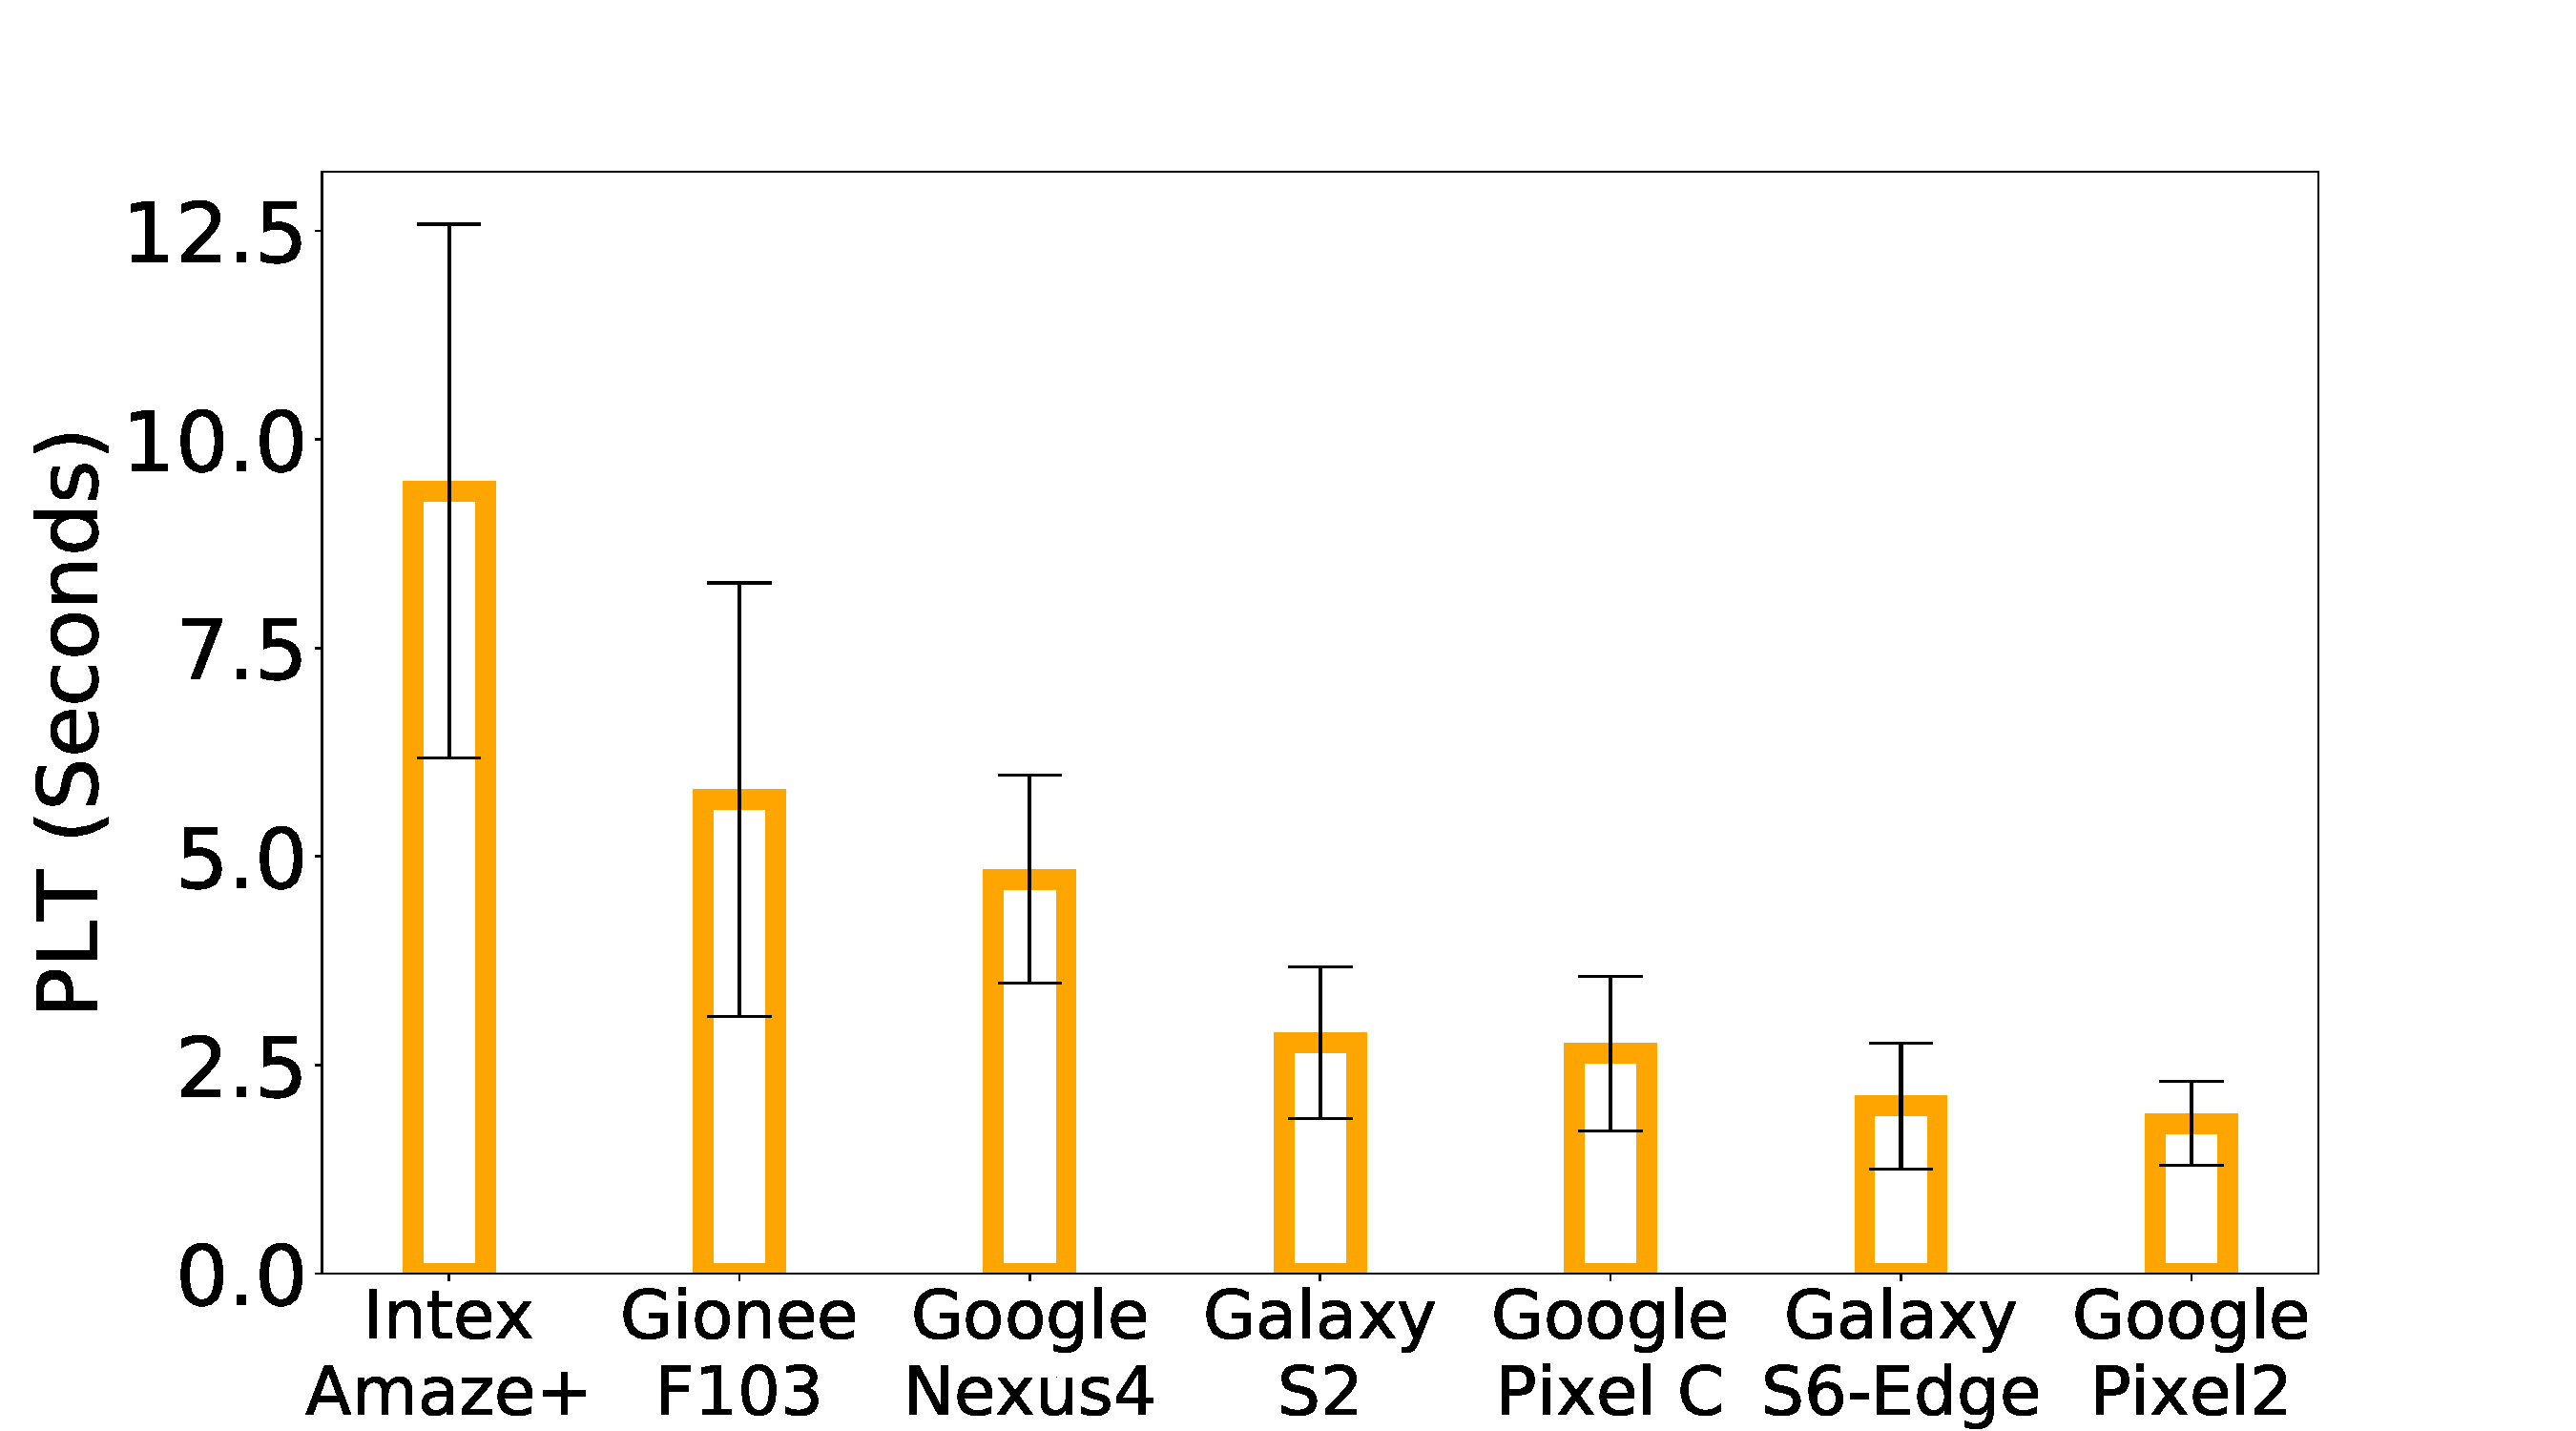
\includegraphics[width=0.33\textwidth]{sections/device-work/plt-devices}
%     }
%     \subfloat[Video Streaming]{%
%       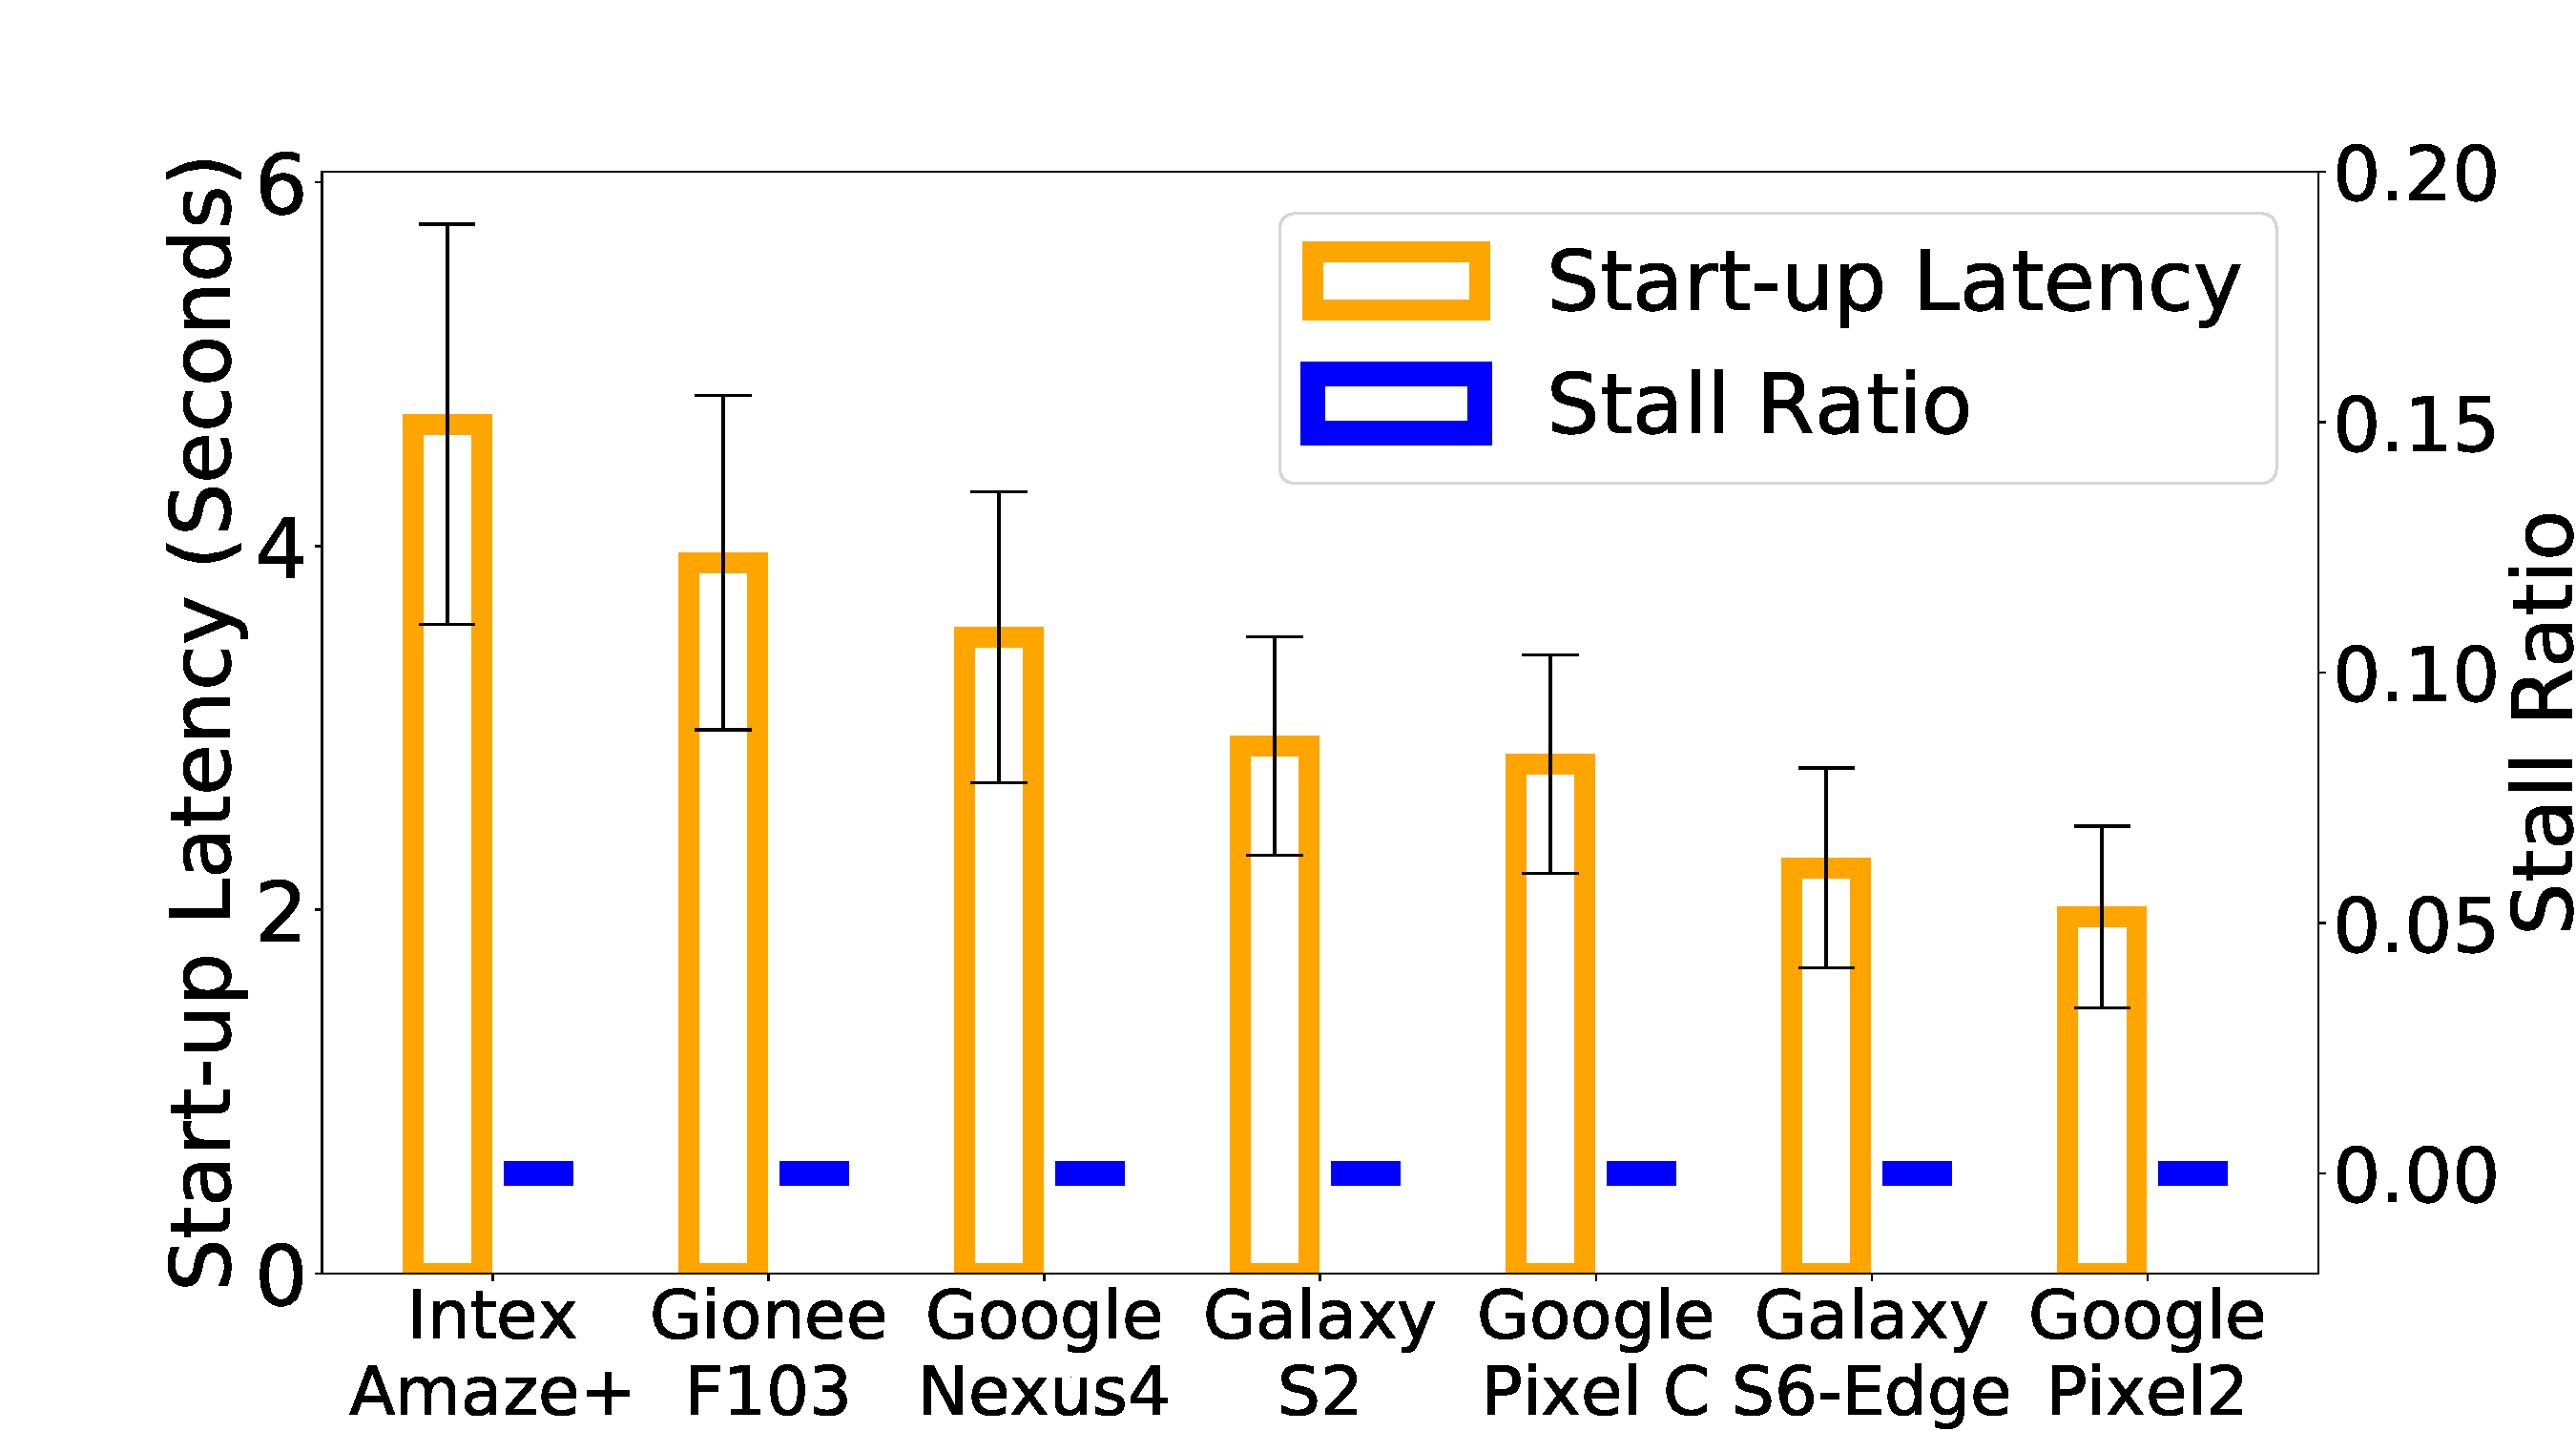
\includegraphics[width=0.33\textwidth]{sections/device-work/youtube-motivation}
%     }
%     \subfloat[Video Telephony]{%
%       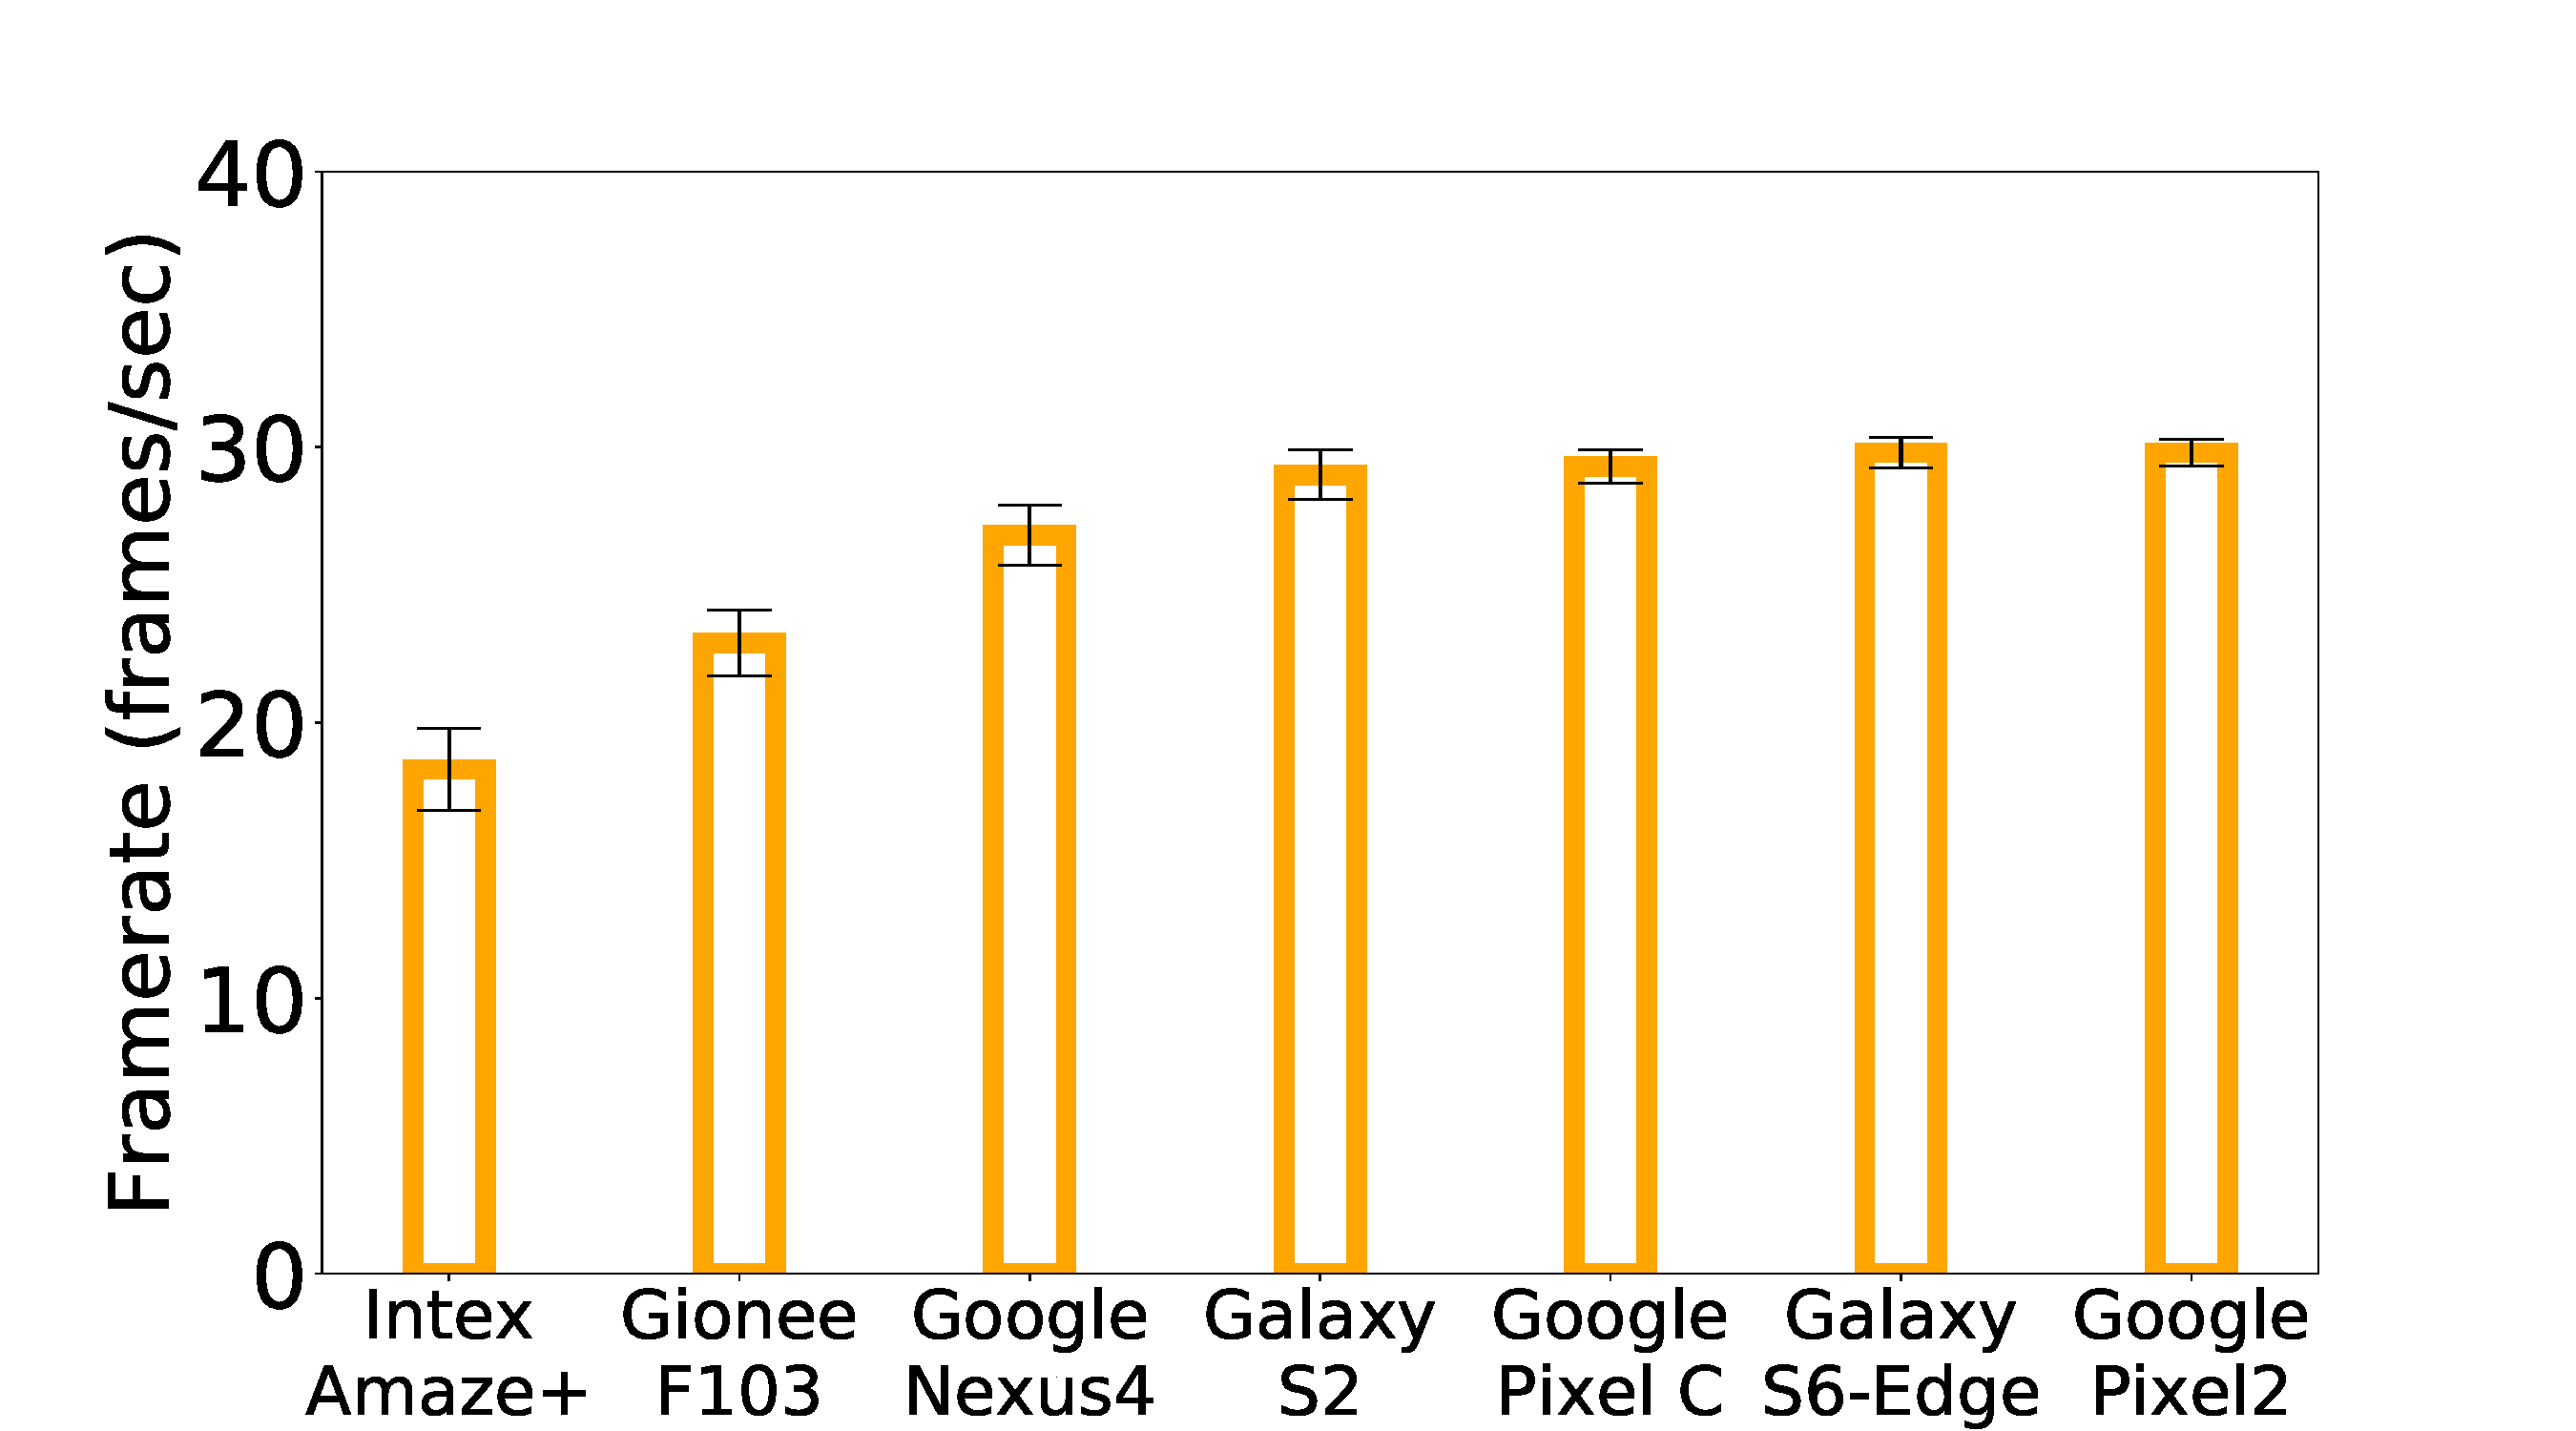
\includegraphics[width=0.33\textwidth]{sections/device-work/skype-motivation}
%     }
%     %\vspace{-0.15in}
%     \caption{Mobile application performance across diverse devices: (a) Web Browsing, (b)Video Streaming, (c) Video Telephony. The horizontal axis shows the device type; their corresponding specifications are tabulated in Table~\ref{tab:device_types}.}
%     %\vspace{-0.2in}
%     \label{fig:motivation}
%\end{figure*}
\begin{table*}[h!]
  \centering
   \scalebox{0.9}{
  \begin{tabular}{c|c|c|c|c|c|c|c}
  \hline \hline
    \textbf{Device} & \textbf{Application} & \textbf{Number} & \textbf{OS} & \textbf{Clock} & \textbf{GPU} & \textbf{RAM} & \textbf{Release} \\
      \textbf{Name} & \textbf{Processor} & \textbf{of Cores} & \textbf{Version} & \textbf{Min-Max (Mhz)}  & \textbf{Type} & \textbf{Size (GB)} & \textbf{Cost} \\
    \hline
    \hline
    Intex Amaze+ &Spreadtrum SC9832A&4&6.0&300-1300 &Mali-400&1&\$60\\
    Gionee F103 &MediaTek MT6735&4&5.0&300-1300 &Mali-T720&2&\$150\\
    Nexus4 &Snapdragon S4 Pro&4&5.1.1&384-1512 &Adreno 320&2&\$200\\
    SG S2-Tab &Exynos 5433&8&5.0.2&400-1300 &Mali-T760&3&\$450\\ 
    Pixel-Tab &Tegra X1&4&8.0.0&204-1912& Maxwell&3&\$600\\ 
    SG S6-edge &Exynos 7420&8&6.0.1&400-2100 &Mali-T760&3&\$880\\
    Pixel2 &Snapdragon 835&8&8.0.0&300-2457 &Adreno 540&4&\$700\\ \hline \hline
  \end{tabular}
    }
  \caption{The table shows the set of diverse mobile devices used in our motivation experiment and their corresponding specifications including cost, CPU capabilities, and memory capacity. }%Mobile Devices in our Experiments showing OS/Hardware Specifications: Shown are parameters that impact the performance of mobile applications}
  \label{tab:device_types}
\end{table*}


%\aruna{add something about the significance of these observations}

%We aim to develop a systematic methodology and analyze hardware and software performance of smartphones. We first study the network performance in smartphones with respect to different device characteristics with a longitudinal data. Then, we focus on mobile Internet QoE with respect to device performance based on hardware parameters i.e, Quality of Service (QoS). We target three popular mobile Internet applications: 1) Mobile web browsing is proven to be constrained by device capabilities over network capacity \cite{nejati2016depth}. We investigate this poor mobile web performance and identify critical factors. 2) File download is also another most used Internet application for which the download time should as small as possible. Although the network is the dominant factor for this application, we observe a significant change in download performance with respect to device capabilities. 3) Video streaming and telephony is computationally intensive because of decoder complexity. We identify the QoE parameters for these applications and investigate the performance with respect to QoS. We observe a significant change in the impact of device performance on all three applications.



%This motivates us to understand the impact of hardware bottlenecks in mobile Internet QoE for low-end mobile users. We believe this work provides consumers, application developers, vendors and content providers in improving the mobile QoE. In this work, we show evidence to suggest that computation bottlenecks are still present in high-end mobile devices and it becomes far worse for low-end mobile devices.

%Unlike desktop-based Internet applications, whose performance is mostly constrained by just the quality of the network, mobile Internet applications face challenges in multiple dimensions: the network characteristics and the underlying software and hardware capabilities. Understanding the performance of mobile Internet applications is useful in assisting: 1) end-users to choose the best suitable smartphone, 2) application developers to make optimize the software, and 3) Vendors to optimize the architecture and operating system for better application Quality of Experience (QoE). At the same time, the service providers can use this knowledge in customizing the content for smartphone users. A lot of work has been there in understanding the impact of the network on mobile Internet applications \cite{Ruamviboonsuk:2017:VAM:3098822.3098851, kelton2017improving, sun2016cs2p}, while a little is there on hardware and software impact. Understanding device impact is quite challenging due to a lack of a systematic approach for controlled experiments and comparative analysis. Our work tries fill this gap.



%Often, the smartphone application processor has a combination of co-processors: a Central Processing Unit (CPU), Graphics Processing Unit (GPU), Digital Signal Processor (DSP) and Image Signal Processor (ISP). Mobile applications such as video and web exploit these heterogeneous devices in offloading the CPU computation, improving the performance and optimizing/scarifying power consumption. The application performance improvement heavily depends on how efficiently one exploits the co-processor (e.g, video decoding can be completely offloaded to GPU or DSP, but web browsing is hard to efficiently offload because of lack of concurrency).

%We find a significant impact of CPU clock frequency and load on different mobile applications.
%For example, we look at the performance of three applications -- file download, web browsing and video transport.
%Reducing clock frequency from $1512 \ Mhz$ to $384 \ Mhz$ slows down file download time an average of 3 times at a CPU load of $50\%$.
%Under the same conditions, the web page load slows down by an average of 4 times.
%Furthermore, we find that a reduction in processor performance hurts web browsing by slowing down both its downloading and compute requests.
%It reduces network throughput, which forces the browser to wait longer for the data.
%It also directly slows down the browser's scripts due to its slower processing.

%Interestingly, we do not observe this effect for video transport. For instance, video streaming (YouTube) has almost zero effect of clock frequency while Skype has some effect though not as much as web browsing. This is despite the fact that video applications impose much higher computation demand on the mobile hardware than file download and web browsing. We find that this discrepancy in performance occurs largely due to efficient offloading of decoding to the GPU processor. Unlike video transport, web browsing is not offloaded to coprocessors and thus its performance is affected more by the processor. Therefore, we investigate this direct impact of hardware on applications as well as indirect impact of hardware through network.



%We summarize the contributions of this paper as follows:
%\begin{itemize}
%\item An in-depth study of device performance impact on mobile Internet QoE. We find web browsing is greatly effected compared to other applications.
%\item We investigate the direct and indirect effect of hardware on these applications.
%\end{itemize}
